% Options.
%
% Language
%  en  -  english (default)
%  de  -  german
%
% Modes
%  draft     - drafting mode, esp for todos
%  fulldraft - drafting mode, also for listings/graphics, faster
%  final     - final mode
%
%
% Fonts
%  lmodern   - Latin Modern, like TeX default
%  palatino  - Heavier, slightly more readable (default)
%  garamond  - Lighter than palatino, heavier than latin modern, more readable.
%
% Other
%  print - do not color links
%  zebralistings - alternating row colors for listings
%
\documentclass[draft,master]{swathesis}
\usepackage[backend=biber]{biblatex}
\addbibresource{thesis.bib}

\usepackage{titlepage}
\TitlePageStyle[
subject=master,degree={Master of Science},
]{hpi-swa}

\supervisors{%
Prof.\,Dr.\,Robert Hirschfeld\and %
Dr.\,John Doe%
}

% ABGABEDATUM
% \setdate{2012}{04}{05}
% \date{\datedate}

\author{Daniel Stolpe}
\location{Berlin}
\extratitle{\raggedleft Stolpe, \\ GraalLSP\par}

\title{A Language Server for Truffle-based Programming Languages}

% LSP + Graal focused
\title{GraalLSP: A Language Server for the GraalVM}
\title{GraalLS: A Generic Language Server for the Truffle Framework}
\title{GraalLS: A Language Server for Language Implementation Frameworks}
\title{GraalLS: A Language Server for Interpreter-based Language Implementation Frameworks}

% Graal focused
\title{GraalLS: IDE-agnostic Tooling for Truffle-based Programming Languages}
\title{GraalLS: IDE-agnostic Tooling for Graal/Truffle-implemented languages}
\title{GraalLS: IDE-like Tooling for GraalVM-supported Programming Languages}

% Langauge Implementation Framework focused
\title{GraalLS: A Language-agnostic IDE for Language Implementation Frameworks}
\title{GraalLS: IDE-like Tooling Support for Language Implementation Frameworks}

\title{GraalLS: IDE-like Tooling for Performance Focused Language Implementation Frameworks}
\title{GraalLS: Getting IDE-like Tooling for Performance Focused Language Implementation Frameworks with minimal effort}

\title{GraalLS: IDE-agnostic Tooling for Programming Languages Built with High-performance Focused Language Implementation Frameworks}

\title{GraalLS: Developing Fast and Tooling-rich Programming Languages}
\title{GraalLS: Developing High-performing and Tooling-rich Programming Languages}

\title{GraalLS: Language-agnostic * from runtime feedback}
\title{GraalLS: Language-agnostic * from runtime feedback}
\title{GraalLS: Zero-overhead LSP implemenation for the GraalVM}


\title{GraalLS: Using runtime feedback }
\title{GraalLS: Towards free IDE support}
\title{GraalLS: Automatic IDE support from runtime }


\title{GraalLSP: A Zero-overhead Polyglot Language Server Implementation for the GraalVM}

%\subtitle{Ein Untertitel ist Optional}
\othertitle{Ein Language Server für Truffle-basierte Programmiersprachen}
\othertitle{GraalLSP: Eine Overhead-freie Language Server Implementierung für die GraalVM}
%\othersubtitle{This is Optionally Optional}

\begin{document}
\frontmatter
\maketitle
\begin{abstract}
  An increasing number of companies build their business on
  distributed Web applications. Hosting providers respond to that
  demand and made it easier to deploy systems that spread across
  multiple services. However, this trend has outpaced the development
  of adequate debugging tools and developers still have to rely on an
  improvised patchwork of symbolic debuggers and printf debugging to
  find failure causes.

  Consequently, observing and debugging failures in distributed
  applications is laborious and time consuming. As multiple processes
  execute in parallel, developers cannot systematically stop and
  inspect the entire system. Although processes are implemented in
  different languages, and often tightly coupled, debugging tools that
  span across processes and languages are practically
  non-existent. Instead, developers have to use different debugging
  techniques to inspect each process sequentially. This makes it hard
  to reason about causality, because the network communication changes
  when debugging a process. That may lead to failures that occur in
  deployed systems, but that developers cannot reproduce locally.

  This work presents an integrated method to support debugging of
  distributed systems in four steps: First, we continually trace
  network communication to have accurate data about event order if a
  failure occurs in a deployed system. Second, we compare
  communication patterns heuristically to identify anomalous
  differences and guide developers in search of failure causes. Third,
  we replay failing network schedules to reproduce failures in a local
  test environment. Finally, we refine the traced data during replays
  and connect network events to code locations. We present network
  events and code within one tool, so developers can use both levels
  of abstraction for debugging.

  We show how our approach can be used to inspect failures in
  distributed systems that would be hard to debug with traditional
  approaches.
\end{abstract}

\begin{zusammenfassung}
  Die Zahl der Firmen, die als Teil ihres Geschäftes verteilte Web
  Anwendungen entwickeln, nimmt zu. Anbieter zur Bereitstellung von
  Servern bedienen die steigende Nachfrage, und erleichtern den
  Einsatz von Systemen die sich über mehrere Dienste hinweg
  erstrecken. Dieser Trend jedoch schreitet schneller voran, als die
  Diagnoseprogramme für diesen Einsatzbereich weiterentwickelt werden,
  weshalb Entwickler noch immer mit symbolischen Fehlersuchwerkzeugen
  und Protokollierung arbeiten müssen, um Fehler zu finden.

  Folglich ist das Beobachten und Beheben von Fehlern in verteilten
  Systemen noch immer mühselig und zeitaufwendig. Da mehrere Prozesse
  parallel laufen, können Entwickler nicht das gesamte System zur
  Untersuchung anhalten. Obwohl Prozesse in mehreren Sprachen
  implementiert, und eng gekoppelt sind, gibt es praktisch keine
  Werkzeuge, die über Prozess- und Sprachgrenzen hinweg
  funktionieren. Stattdessen müssen Entwickler verschiedene
  Fehlersuchtechniken für jeden Prozess einzeln anwenden. Das
  erschwert es ihnen, kausale Zusammenhänge zu verstehen, da sich das
  Kommunikationsverhalten ändert, wenn einzelne Prozesse untersucht
  werden. Das kann dazu führen, dass Fehler, die im Produktivsystem
  auftreten, von Entwicklern lokal nicht reproduziert werden können.

  In dieser Arbeit wird eine Methode zur Fehlersuche in verteilten
  Systemen präsentiert, welche die folgenden vier Schritte umfasst:
  Zunächst wird fortwährend die Kommunikation im Netzwerk
  aufgezeichnet, um im Falle eines Fehlers im Produktivsystem den
  Entwicklern akkurate Ereignisdaten bereitzustellen. Daraufhin werden
  diese Daten mithilfe einer Heuristik auf Anomalien in den
  Kommunikationsmustern hin untersucht. Weiterhin werden diese Daten
  zur Wiedergabe der Kommunikation in einem Entwicklungssystem
  genutzt. Schließlich werden die aufgezeichneten Daten während der
  Wiedergaben verfeinert, und so die Netzwerkdaten mit dem Quelltext
  assoziiert. Beides wird in einem Werkzeug präsentiert, sodass
  Entwickler beide Abstraktionsebenen zur Fehlersuche nutzen können.

  Wir zeigen wie unsere Methode genutzt werden kann, um Fehler in
  verteilten Systemen zu finden, die mit traditionellen Ansätzen nur
  schwierig untersucht werden können.
\end{zusammenfassung}
 

%%% Local Variables: 
%%% mode: latex
%%% TeX-master: "thesis"
%%% End: 

% !TEX root = Stolpe_2018_Thesis.tex
% !TEX encoding = UTF-8
\begingroup
\let\raggedsection\centering

\chapter*{Acknowledgments}
\label{cha:acknowledgments}
\endgroup
\begin{quotation}
  \noindent I owe everything to my cat.
\end{quotation}
%%% Local Variables:
%%% mode: latex
%%% TeX-master: "Stolpe_2018_Thesis"
%%% coding: utf-8
%%% End:

\tableofcontents
\listoffigures
\listoftables
\lstlistoflistings
\listofacronyms %
\mainmatter
% HAUPTTEIL
% \chapter{Introduction}
\label{cha:introduction}

From its beginnings in the 1990s, the Web has become an important
application platform in less than one and a half decades. Industry
surveys indicate that an increasing number of companies develop
distributed Web applications as a core part of their
business~\cite{kondo2009cost,EYPaaSSurvey2012}. However, many of those
applications are not written with distributed systems middleware to
handle communication between services. Instead, developers improvise
their own communication interfaces. This is error-prone and
complicates integration~\cite{Nadiminti}.

Distributed applications are especially prone to software
failures. Recent studies~\cite{Ballou2008,Tassey2002} show a relative
increase in code problems, hidden dependencies, and accidental
complexity when integrating multiple systems. Different systems may
provide different network interfaces and developers need to understand
their utilization and implicit assumptions. Different systems also run
different frameworks and programming languages, so that developers
need help to associate observed network communication with code
locations. This additional complexity makes it harder for developers
to reason about the system as a whole, thus, they are more likely to
introduce defects~\cite{zeller2009programs}. Debugging the resulting
failures is hard, and we have identified four primary problems that
developers face with current approaches and tools.

First, reliably reproducing failures is hard. Since distributed
systems execute in parallel, a global event order is difficult to
establish and may vary non-deterministically across
executions~\cite{lamport1978time}. Such variance depends on the
physical connections between the servers. The development setup will
differ from deployment and, thus, network delays and probabilities for
non-deterministic behavior also differ. Consequently, developers may
not be able to trigger some failures during development that occur in
deployment, or such failures may occur so rarely that it is impossible
to debug them effectively, because developers cannot reliably
reproduce them.

Second, developers cannot easily distinguish between causes and
effects. Many developers rely on systematic logging to understand
failures that only occur during
deployment~\cite{zeller2009programs}. However, isolated event logs are
poorly suited to create a global view on the events in a distributed
application. The ability to reason about global event order is
necessary for humans to understand causality in a
system~\cite{lamport1978time}. Understanding the cause of a failure is
essential for fixing it correctly.

% Consider a search engine. For a small scale engine, developers can
% control data storage, transactions, and database connections. On the
% Internet, the primary communication protocol is \ac{http} which limits
% in the amount of control developers have over their systems'
% connections. Non-atomic data updates usually cannot be wrapped in
% transactions. Storage services on the Web cannot provide transactions
% to thousands of users in parallel. Parallel \ac{http} request are each
% stateless and provide no guaranteed ordering. Thus, developers can
% rely less on the underlying infrastructure and require debugging tools
% work in a distributed setting.

Third, developers cannot easily inspect execution on servers in the
system. With symbolic debuggers, programmers inspect execution state
and behavior to find anomalies that may have caused a
failure. Symbolic debuggers enable them to stop execution and
interactively inspect the program's state. However, in a distributed
system, developers need to inspect state across multiple servers,
which execute in parallel. Symbolic debuggers are tailored towards
systems under developer control, but not all parts of a distributed
system provide that kind of control. Stopping servers with a debugger
to inspect the execution state is not feasible during deployment and
external services may not provide any debugging mechanism.

Finally, different frameworks and programming languages on several
servers force developers to apply multiple debugging
tools. Consequently, developers cannot debug and inspect the
distributed system as one. Instead, they have to treat each system
separately, because current debugging tools cannot connect and
synchronize with others. Support for debuggers that work across
multiple servers and languages is virtually non existent.

Due to these problems, debugging failures in distributed systems,
especially non-deterministic failures, is a time-consuming task. It
usually consists of aggregating various forms of log files, debug
output, and \ac{api} documentation for the employed services, and then
debugging on an equivalent, local system to infer possible
problems. Symbolic debuggers cannot be used in distributed
applications, because they only support independent analysis of
individual processes and require full control over those.

Tool support for network observation, log aggregation and debugging
across different systems is virtually non-existent. Yet, to improve
programmer productivity, providing adequate debugging tools is a key
ingredient, as without them, debugging is a manual, time-consuming
task~\cite{Dinning1990}.

We argue that there is a need for debugging tools that target
distributed, heterogeneous systems which are not entirely under
developer control. Architectural patterns for the these kinds of
systems, such as \ac{soa} and \ac{rest}; and hosting services, such as
\ac{paas} and \ac{iaas}, are relatively new phenomena---the first
comprehensive description of \ac{soa} was in 2005~\cite{Erl2005}. For
that reason, much of the work in this area is still not aimed at the
specific challenges of debugging distributed applications. Developers
of these systems need tools that provide a means to record and replay
events consistently across multiple servers. The tools should
furthermore guide developers towards anomalous differences across
multiple executions, so developers can reason about causality in the
system. Finally, such a tool should allow developers to cope with
multiple frameworks and languages, as they are common in distributed
applications.

\section{Approach}
\label{sec:approach}

In this work we present an approach for integrated debugging in
distributed applications, targeted specifically at Web development,
but extensible to other kinds of applications with similar
problems. Our approach---Replay-driven Fault Navigation---combines
state of the art techniques in the area of record and replay to
eliminate of non-determinism, distributed program comprehension, and
statistical debugging.

To allow debugging of non-deterministic failures, we present a tracing
approach for unified monitoring of systems. We continuously monitor
the live system and record enough data to allow reproducing relevant
program state at a later time. Our monitoring imposes little overhead
so it does not disturb execution unduly and can stay enabled during
deployment. We analyze the recorded data and correlate it to failures
to determine causes and effects. Network schedules are treated as
sequences of send and receive events between pairs of servers. Our
heuristics assign cause probabilities to sub-sequences of the recorded
network schedules, to guide developers during debugging. Developers
can replay such event sequences with our network scheduler and
iteratively refine recorded execution data for inspection. The
scheduler is an intermediate layer that controls how network events
pass between the application code and the framework. It blocks or
stalls events to change the order in which they pass in and out of the
application to match the recorded sequence. We correlate the network
data with source code and present both in a unified debugging tool, so
developers can debug at either level of abstraction and correlate
source code across servers and languages.

The advantages of our approach over traditional stop-the-world
symbolic debuggers are: the impact on the runtime behavior is kept at
a minimum, the technique can be applied to the live system,
eliminating the need for a test setup, and the debugging tools can
help developers to logically connect source code locations across
different servers.

To our knowledge, the presented approach is unique in that it
explicitly tries to support debugging across different languages and
system with one integrated approach. Work on understanding and
debugging distributed systems has been on-going for some
time~\cite{Parker1983} and the state of the art has solutions for each
part of Replay-driven Fault Navigation, but no integrated solution
exists that we are aware of.

\section{Outline}
\label{sec:outline}

This work is structured as follows: in \autoref{sec:requ-based-distr},
we discuss the problem domain on a small example. We highlight
challenges faced by developers when working with current debugging
techniques. In \autoref{cha:solution-design}, we present our four-step
approach to those challenges, and how that approach could work in
different languages and deployment scenarios. In
\autoref{cha:implementation}, we discuss an implementation of
Replay-driven Fault Navigation in Smalltalk. Finally in
\autoref{cha:evaluation}, we use the initial example and a larger
application adapted from an industrial system to evaluate our tool in
comparison with contemporary techniques. In
\autoref{cha:related-work}, we discuss related work and present our
conclusions in \autoref{cha:conclusion}.

%%% Local Variables: 
%%% mode: latex
%%% TeX-master: "thesis"
%%% End: 

% \input{context}
% \input{solution}
% \chapter{Implementation}
\label{cha:implementation}

\begin{figure}
  \centering
  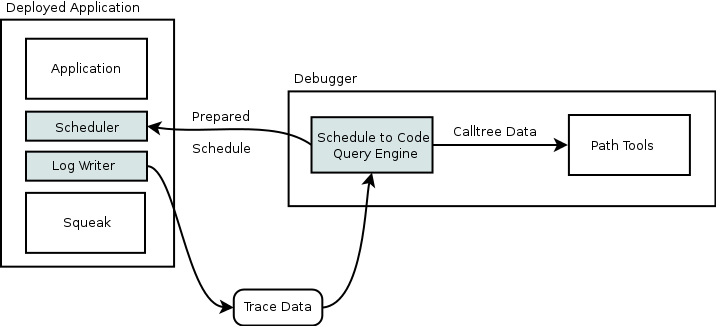
\includegraphics[width=0.9\linewidth]{structure}
  \caption{Interactions in the Prototype}
  \label{fig:structure}
\end{figure}

We evaluated our approach in a prototype for distributed applications
using \ac{http} to communicate, implemented in
Squeak/Smalltalk~\cite{Ingalls1997}. In this chapter, we explain how
we hooked into the entry and exit points for network communication,
for which we used \emph{ContextS}~\cite{Hirschfeld2008}, an
implementation of \ac{cop} for Squeak/Smalltalk. We already mentioned
that we built on earlier work about online analysis of runtime
behavior, implemented in the \emph{Path Tools} suite, and we have
based our debugging tool and visualization on the Path Tools
suite. \autoref{fig:structure} shows how our protoypes' components
interact. Applications are instrumented with ContextS to include a
logging and a scheduler layer. The logging creates trace data that is
used by our query engine to display the network communication patterns
with the Path Tools and provide any recorded call tree data. When the
developer chooses a schedule for re-execution, queries are attached to
the schedule events, the prepared schedule is sent to the scheduler,
and the application is re-executed. The scheduler shapes the
communication during re-execution to match the schedule and records
any additional information using the same mechanism as the log
writer. The resulting trace data is again sent to the query engine,
which passes the newly recorded information to the Path Tools for the
developer to inspect.

\section{Tracing Communication Patterns}
\label{sec:trac-comm-patt}

One way to implement the logging of logical communication schedules is
tracing the appropriate code executions in the system. For our
application, we identified the methods in a Squeak image where
\ac{http} requests are received and responses are generated. Our
example application used, besides the standard library \ac{http}
communication, the \emph{KomHttpServer} for receiving requests.

Tracing communication at different levels of granularity was vital to
verify our approach in a prototype. We chose ContextS so we could
easily add various layers with different logging mechanics for
experimentation. Additionally, ContextS layers are easy to manage in
Monticello, the \ac{vcs} of Squeak. This allowed us to keep the
tracing implementation as a separate project an thus fairly
independent of the traced system.

The combined log includes all events that were recorded between two
particular points in time. These points in time are given by the start
and finish of our diagnosis to reproduce a failure. Re-executing such
a diagnosis a number of times yields different time slices of
communication. We present these logs in a diagram with events as data
points and logical time on the x-axis. Because events are data points,
and there may be many events in one schedule, our visualization scales
all events to fit into one window. For many events, this allows
developers to get a high-level overview of the activity throughout the
system without swamping with detail. In \autoref{fig:comm-overview} we
see such an overview. While we cannot make out details, we can see
that the service running on \emph{localhost} port 5001 is active more
consistently than the one below it, running on port 5002. This
high-level pattern communication pattern may already provide some
insight as to how the system works.

\begin{figure}
  \centering
  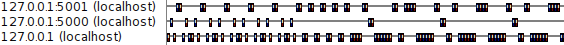
\includegraphics[width=0.95\linewidth]{comm-overview}
  \caption{Communication Schedule Overview}
  \label{fig:comm-overview}
\end{figure}

\autoref{fig:comm-logs} shows an example of a very small communication
schedule. We show the number of diagnosis runs that yielded this
particular schedule (\textcircled{1}), and how many events there are
in this schedule. The color of the box shows whether there were any
errors, such as failed assertions, during the diagnosis' execution by
turning from green to yellow. The recorded communicating servers
(\textcircled{2}) are presented as \textsc{IP} address labels on the
y-axis, with the associated port (if any). If that address resolves to
a host name, it is added in brackets. \emph{Lifelines} extend from the
endpoints, so events on the right-hand side can be easily associated
to a particular server. Each box represents an event with outgoing
events (\textcircled{3}) in red and incoming events (\textcircled{4})
in blue. The boxes in this visualization represent a point in time
rather than a time span, and their width is simply as wide as possible
to still show all events within the graph. Because each box shows the
first few bytes of captured message data if such has been captured, it
is useful to have boxes as wide as possible.

\begin{figure}
  \centering
  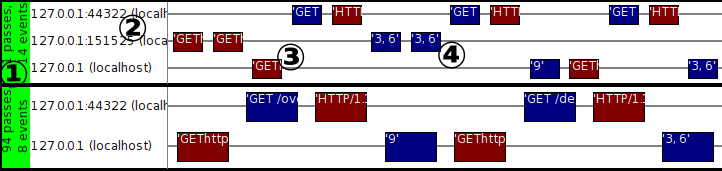
\includegraphics[width=\linewidth]{comm-log}
  \caption{Captured Communication Logs}
  \label{fig:comm-logs}
\end{figure}

\subsection{Distributed Context-oriented Computing}
\label{sec:distr-cont-orient}

ContextS layers can be dynamically enabled and disabled to extend
methods at runtime. For a distributed system, these layer activations
have to be distributed across the network, so enabling a particular
tracing mechanism on one system carries over to another. This can be
achieved in various ways. Because our layers are implemented for
\ac{http} requests only, we decided to propagate layers in a custom
\ac{http} header, \texttt{X-DCOPActiveLayers}, an application specific
header in accordance with RFC 2047. This header contains not the names
of the currently active layers, but, as suggested in~\cite{Rho2011},
an ontology describing those layers. This decouples the layer names on
our particular implementation from possible other implementations and
their layer names, by describing what layers do instead. Those headers
will be ignored by conforming implementations that do not use our
tracing package. On systems that do use our tracing, we read the list
and activate the layers globally as required.

Most Web application frameworks employ the \emph{inversion-of-control
  principle}, which does not work well for ContextS. In ContextS,
layer activations are valid for the dynamic scope of the execution,
and do not propagate upwards the stack from the point of
activation. This problem with \ac{cop} in the context of
inversion-of-control frameworks is known and has been treated in
recent work~\cite{Appeltauer2012,Appeltauer2012Phd}. We have not
implemented the mechanism to deal with this problem, so our prototype
is not able to activate layers across the network. Rather, the
required layers are simply active all of the time.

In related work, DejaVu uses a similar mechanism on the transport
layer that involves embedding and, on the remote end, stripping magic
bytes in \ac{tcp} packages~\cite{Konuru2000} to propagate
meta-information for tracing.

\subsection{Tracer Entry Points}
\label{sec:tracer-entry-points}

Tracing \ac{http} requests with ContextS entails finding and layering
methods in frameworks and standard library that create and receive
\ac{http} requests. In our example, using the Squeak standard library
and the KomHttpServer framework, this included layering only 3
methods.

Extending the implementation to work for other Squeak Web servers or
other application layer frameworks such as relational database
adapters is trivially possible. The actually captured data only
includes the local logical timestamp, as well as the sender and
receiver of the message.

\subsection{Trace Format}
\label{sec:trace-format}

To actually implement our approach for different runtimes and debug
across languages, an interchangeable trace format is necessary. We
have not implemented such a format. Our prototype is Squeak-based, so
the interchange format consists of a Squeak store string, which can be
recompiled into a collection of trace events. Each trace event, here,
is an object with a logical timestamp, receiver and sender \textsc{IP}
and port.

An interchangeable trace format is trivial to implement, however. To
exchange logs, we only need a way to transfer collections of event
3-tuples that include strings and integers which almost any
data-interchange format should be able to. \ac{json} seems to be a
natural choice, both because it is widely used and parsers are readily
available for a variety of languages, and because it is the most
common format in Web development.

\section{Communication Diffing}
\label{sec:diff-comm}

As per our design (\cf{\autoref{sec:comm-constr-analys}}), we regard
each communication schedule as a sequence diagram with only
asynchronous message sends. To help developers find differences in the
schedule, we want to automatically differentiate traces to show areas
of high and low variance in the schedule. For $N$ servers, at any one
logical time, there are at most $N$ network events. Comparing
different communication schedules can thus be done by comparing each
logical time in order, similar to how a patch algorithm compares files
at different versions.

\subsection{Difference Format and Visualization}
\label{sec:diff-form-visu}

The choice of algorithm for automatic differentiation can have a huge
impact on the usefulness of the result. There are various algorithms
to differentiate tree structures~\cite{Bischof2008AiA}. We treat our
communication schedules as call trees with only asynchronous
communication. That means they can be transformed into a linear form,
which makes them suited for the linear differential algorithms used
for file comparison. Of those, we chose the \ac{lcs} algorithm to
create differential schedules.

We can assume that schedules will vary in some events or
event-sequences, but will be equivalent for some length around those
variances. \ac{lcs} dynamically finds the longest matching
sub-sequence between two pieces of data. For comparing two schedules,
we choose one as the \emph{base} and the other as the change. In
\autoref{fig:comm-diff} we show such a differential schedule between
the base at the top and the comparison schedule at the bottom.

The differences between the schedules are marked in red. If we compare
the overall number of events, we can see that both the base schedule
at the stop and the comparison schedule at the bottom have the same
number of events. They are equivalent up to the first red marker,
where the comparison schedule sends out a \texttt{GET} request that
does not occur in the base schedule. If we follow the differential,
however, we can see that the schedules are equivalent again for four
more events until the second red marker. At that point, a \texttt{GET}
request sent in the base schedule does not occur in the comparison
schedule. Afterward, both are equivalent up to the end.

\begin{figure}
  \centering
  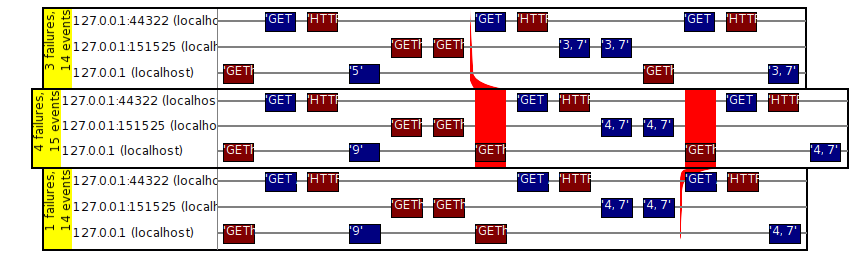
\includegraphics[width=\linewidth]{comm-diff}
  \caption{A Simple Differential Between 2 Schedules}
  \label{fig:comm-diff}
\end{figure}

\subsection{Correlating Variances and Failures}
\label{sec:corr-vari-fail}

Not all variances will usually contribute to the failure, yet, for
large numbers of runs we may have more variances than common
sub-sequences. Simple red/white differentials are not very helpful in
this case, as they do not significantly reduce the search space to aid
developers in their search for the problem. Due to this, we weigh
variances according to a number of rules, which have been in described
in \autoref{sec:assoc-vari-with}.

The heuristic probability distribution is mapped onto hue values from
zero to sixty degrees, which corresponds to full red and full yellow,
respectively. For variances that the heuristic recognizes to have no
impact on the failure, we assign the color gray.

To review variances between passing runs, we assign hue values
depending on the amount of variance on each particular network
event. The function \emph{hue}, below, shows how we map the each event
onto a range from 0 to 1. We then map this range onto a range from 0
to 60, corresponding to the colors from red to yellow in the
\textsc{hsl} color space. We assign alpha values from 0 to 1
accordingly, which means that events with a hue closer to 60 are
hardly visible.

\begin{align*}
  \label{eq:1}
  T & = \text{set of trace event sets} \\
  N(event) & = \{ T_{i} \in T | event \in T_{i} \} \\
  P(event) & = \{ T_{i} \in N(event) | T_{i} \text{ is pass} \} \\
  hue(event) & = \left\{
    \begin{array}{l l}
      \left(1 - \frac{|N(event)|}{|T|}\right)^2 & \qquad \text{if } N(event) = P(event) \\
      \sqrt[12]{\left|0.5 - \frac{|P(event)|}{|N(event)|}\right|} & \qquad \text{else}
    \end{array}
  \right.
\end{align*}

The result of this mapping, shown in \autoref{fig:hue-mapping}, is
that high-variance events from traces that are all passes or all
failures show more red, which in return means that low-variance events
have almost no highlighting. In sets of traces that include both
passes and failures, the second branch of the \emph{hue} function is
used to determine a value that highlights events that occur not in all
passes---thus are not likely to be the cause for passing---but also
not only in failures.

\begin{figure}
  \centering
  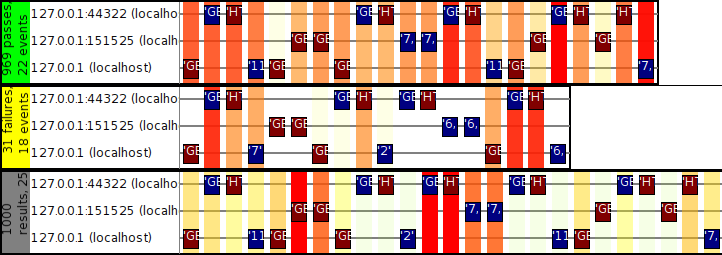
\includegraphics[width=\linewidth]{hue-mapping}
  \caption{Hue Mapping For Events}
  \label{fig:hue-mapping}
\end{figure}

\section{Reordering Access to Network Resources}
\label{sec:reord-access-shar}

In our prototype we support re-scheduling network access in the live
system. Parallel network events inherently cause races, the network
transport may transmit messages at different speeds and the operating
system may forward messages to user space applications as it sees
fit. To reorder access to network resources, the network events have
to arrive at the application in order, so network events have to be
re-ordered in a layer between the application and the hardware.

We decided to re-order events in the language, using the same
mechanism as for tracing. We use ContextS to define a scheduler layer
between applications and the KomHttpServer framework and the Squeak
standard library (\cf{\autoref{fig:structure}}). This scheduler layer
is only active if a schedule was requested.

\subsection{Constraints on the Networked Systems}
\label{sec:constr-netw-syst}

Our design is supposed to work for local systems on the developer
machine, in test environments and the live system. However, because we
only record communication partners and the partial ordering of events,
in practice, there are various constraints on those systems. First,
hey have to be deterministic in their communication, which means if we
send them messages in the right order, they return valid responses in
right order. This means have to be able to control the order in which
messages are received. However, with systems that employ load
balancing, multi-threading and event loops which are designed to
handle multiple requests in parallel we cannot be sure that for
multiple requests the responses are generated in order. This means we
have to control the send order, too.

\subsection{Entry Points}
\label{sec:entry-points}

According to the design, there are two types of entry points which we
need to control to enable re-scheduling, both for sending and
receiving. We only deal with \ac{http} requests and, because we use
the same context-oriented mechanism as for the tracer, we only had to
create a layer to wrap the same three methods as for the tracer. Our
scheduler layer is always active and the wrapper methods check whether
a schedule was requested. This check simply uses a globally available
singleton object and checks whether it contains a valid schedule. If
not, the scheduler methods do nothing and simply proceed.

\subsection{Scheduling Execution}
\label{sec:scheduling-execution}

Our implementation follows the design shown in
\autoref{fig:reorder-sched}. The framework we used to implement our
example application uses threads to handle multiple connections, so
for simplicity, we have only implemented the threading scheduler using
semaphore queues.

To schedule an execution, the trace that is used as basis for the
execution is copied and transformed into a list of schedulable
events. All of these events contain the identifiers for the original
communication partners, the id of the event and a semaphore in the
\emph{waiting} state. This list is then attached to the globally
accessible singleton object and the first semaphore is
signaled. Finally, the diagnosis script is started to provide the
required events.

\paragraph{Receive}
\label{sec:receive}

The KomHttpServer uses a blocking \emph{accept} call on a socket
object to wait for incoming requests, which the \ac{vm} translates
into the \emph{accept} system call. When that call returns, the
operating system socket has data available. The KomHttpServer
framework then spawns a new thread that creates an
\emph{HttpRequest} object from the received data and passes this
into the application.

Before it passes from framework to application code it has to go
through our scheduler. The scheduler uses an atomic operation to find
the appropriate event in the schedule for this request, attach the
request object onto it, and return the event object from the
schedule. It then calls \emph{wait} on the event object's
semaphore. If the semaphore was already signaled this call returns
directly, otherwise this thread blocks until the semaphore is
signaled.

When the \emph{wait} call to the semaphore eventually returns, the
semaphore for the following event is signaled and the request object
is passed back into the framework, from which it passes on into
application level code.

\paragraph{Send}
\label{sec:send}

Sending of data works similarly. The application manufactures an
\emph{HttpResponse} object and returns it to the framework. The
framework the calls the \emph{writeOn:} method with the socket object
to serialize the response onto the socket stream. We wrap this method
and use the atomic find, set, and return operation on the schedule to
find the scheduled event corresponding to this response, and then wait
on the semaphore. When semaphore is signaled, we proceed to the base
method which writes the response to the network.

The fact that we have only implemented the semaphore list for our
scheduler means that means it is currently limited by the maximum
amount of threads available to the framework for handling multiple
connections. Because each thread blocks if the event cannot be
released directly there may be situations in which so many threads are
blocked that the framework cannot create any more threads for incoming
requests, at which point the server will deadlock. We circumvent this
problem in our implementation by having the semaphore wait time out
after a configurable amount of time, after which point the
re-scheduling deviates from the desired schedule.

\subsection{Probable Replay}
\label{sec:probable-replay}

A goal for a scheduler following our design is to enable consistent
replay. Our design only works for well-behaved clients and stable
networks, constraints that cannot always be guaranteed in a real
environment. However, these constraints may often be met, even if not
all the time. A practical re-scheduler may not always work, but it
raises the probability that a specific schedule will be reproduced,
and it will reproduce the schedule if the circumstances permit. If the
network is sufficiently disturbed, either because of misbehaving
clients or connection problems, the scheduler deals with it by
deviating from the desired schedule.

As mentioned above, our implementation uses timeouts to make sure that
the distributed system does not lock up, but timeouts include the
potential for releasing events too early and thus deviate from the
desired schedule, causing a re-execution inconsistent with the
original trace. Our implementation also continually checks for
disturbances defined in
\autoref{sec:required-heuristics}---unscheduled events, schedule
disruptions by misbehaving clients---and we have implemented
configuration settings that determine how we deal with them. These
settings currently allow developers to choose to drop unscheduled
events, or pass them through without waiting for a semaphore. Our
implementation additionally uses simple printf logging to communicate
to the developers how it is reshaping the network schedule, i.e. which
events have been encountered, which are being waited for, and which
disturbances were encountered and how were they dealt with.

\section{Connecting Network and Object Communication}
\label{sec:conn-netw-object}

Adequate tools are essential for efficient debugging. Previous
approaches at efficient replay for the most part focus on recording
and replaying correctly and efficiently, but use existing debuggers
like \emph{GDB} for interactions with the program state, and separate
tools to review the captured network data. Other approaches, like
\emph{Causeway}, focus on the tools.

We think that the debugging tool should be integrated, allowing the
user to inspect both object and network communication in one view, as
they are in Causeway. However, efficient replay is required for those
tools to be practical, so a recording and replay mechanism like our
scheduler has to be integrated into the tool.

Our prototype extends the call tree view, called \emph{Path Finder},
which is part of the Path Tools suite. Our tool, inspired by Causeway,
shows network communication and the call tree for one server in a
single window. These views should be synchronized, so if a user opens
a method, the closest network event should highlighted. Inversely,
clicking on a network event should open the call tree on the method
that is closest to the network event. If the network event was sent or
received on the server to which the call tree belongs, it should show
the method responsible for the event.

For this prototype, we have only implemented moving from the network
to the code view, not vice-versa. If a user clicks on a network event,
the scheduler is instructed to record the stack at the time of the
network event and the test case is re-executed. We then search for a
method on the stack that is part of our call tree, and open that
method for inspection. In \autoref{fig:pathfinder} we show the result
of clicking on the third network event~\textcircled{1}. In the lower
part of the window, the call tree is expanded to the method which sent
the event.

\begin{figure}
  \centering
  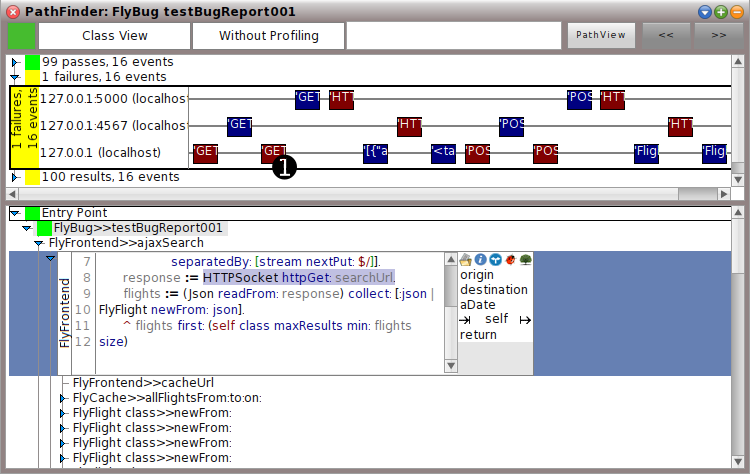
\includegraphics[width=0.9\linewidth]{pathfinder}
  \caption{The Path Finder Network Extension}
  \label{fig:pathfinder}
\end{figure}

A full implementation should support full synchronization between the
two views. We have also not implemented additional queries of the
program state. A fully implemented tool should support queries of
single variable values, method arguments and other program state in
the scheduler, to allow further inspection of the program state.

%%% Local Variables: 
%%% mode: latex
%%% TeX-master: "thesis"
%%% End: 

% \section{Evaluation}
\label{sec:evaluation}

\todolist{tim}{
\item show Sudoku constraints 
\item explain constraints
\item add multiplayer events with constraints (to demonstrate how a
  new codepath does not break the system and ``just works''}
  
  
This section evaluates how well constraint applications with Babelsberg/S facilitate reactive systems.

We argued that logic puzzles, like Sudoku puzzles, are good examples for interactive constraint applications. Therefore, the evaluation uses Sudoku as example application. In \autoref{lst:sudoku-constraints}, you will find all necessary constraints to solve a Sudoku puzzle.

\begin{lstlisting}[caption=All Constraints of a Sudoku Puzzle, label=lst:sudoku-constraints]
sudoku addConstraintsForAllGivenNumbers.

[sudoku allSatisfy: [:cell | cell between: 1 and: 9]] 
		alwaysSolveWith: solver.
		
(1 to: sudoku rowCount) do: [:index |
		[(sudoku atRow: index) allDifferent &
		(sudoku atColumn: index) allDifferent &
		(sudoku atBox: index) allDifferent] 
				alwaysSolveWith: solver].
\end{lstlisting}

The second one, line 3 and 4, was already explained in \autoref{sec:ocp_squeak}. The first line adds equality constraints for all given numbers, so that the constraint solver cannot change them. In general, they are called stay constraints, which are currently not supported in Z3, but will be in future versions. The last constraint, line 6 to 10, describes that all numbers in each row, column and box, are different. The keyword for that is \texttt{allDifferent}, which is a new collection method in Babelsberg/S. Together, the second and third constraint say that each row, column and box contains all numbers from 1 to 9.
% \input{relatedwork}
% \section{Conclusions}
\label{sec:conclusion}

\todolist{tim}{
\item constraints are useful to write reactive systems
\item the relationships between objects are modularized
\item adding new codepaths that affect the relationships works
  automatically}
  
%% softened the conclusion a little - I don't think we have shown this
%% conclusively yet
We have argued that \ac{ocp} facilitates reactive systems, because it
modularizes the relationship between objects and decouples constraint
satisfaction from the application.  In Babelsberg, constraints can be
dynamically added and removed and maintained automatically, making
them useful for writing interactive applications.  As an example, we
implemented an interactive application for specifying and solving a
Sudoku with constraints.  With the interactive \ac{gui}, the user can
change the values of the constraint variables without breaking the
properties of the Sudoku.  The application reacts on the user input by
resolving the underlying constraints.
%%% Local Variables:
%%% mode: latex
%%% TeX-master: "paper"
%%% End:

%

% beispiel.

\chapter{Introduction}
\label{cha:introduction}
\section{Challanges of developing your own language}
    User groups: language developer and language user

    % https://martinfowler.com/articles/languageWorkbench.html
    For a simple example, consider if we want to rename the properties on the target class in my simple example. With a first class modern IDE, automatic refactorings for renaming are habitual. But such a rename won't propagate into the DSL. There is what I'll call a symbolic barrier between the world of C\# and the file mapping DSL. We can translate our mapping into C\#, but the barrier limits our ability to manipulate the overall program.
    This lack of integration hits us in lots of ways with tooling. Firstly - how do we edit our DSL? A text editor will do the job - but modern IDEs increasingly make text editors look primitive. I should get a pop-up list and completion on the field names, red squiggles if the character ranges overlap. But to do this I need an editor that understands the semantics of my DSL.
    Maybe I can live without a semantic editor. But then think about debugging. My debugger can step into the C\# translations, but can't get into the true source itself. What I really would like is a full-blown IDE for my DSL. In the days of text editors and simple debuggers this wasn't a big issue - but we now live in a post-IntelliJ world.
    % https://martinfowler.com/articles/languageWorkbench.html

\section{Language implementations - performance vs. tooling support}
Graal/Truffle: Performance first \cite{grimmer2015high}. Tooling is enabled through instrumentation \cite{van2015building}.
\section{Contribution of this Thesis: GraalLSP}
    This thesis proposes the idea to build a common language server for programming languages implemented with the Truffle framework.
    For the language developer: Reduce the amount of work (can focus on language development, not tool development)
    For the language user: Broader choice in tooling (any LSP client) + more consistent tooling experience for all Graal/Truffle-implemented languages
\section{Structur of this Thesis}


\chapter{Context}
\label{cha:context}

\section{Graal and Truffle}
\subsection{GraalVM}
    GraalVM\cite{graalvm2018} is a high-performance polyglot VM.

    %https://www.graalvm.org/
    GraalVM is a universal virtual machine for running applications written in JavaScript, Python 3, Ruby, R, JVM-based languages like Java, Scala, Kotlin, and LLVM-based languages such as C and C++.

    GraalVM removes the isolation between programming languages and enables interoperability in a shared runtime. It can run either standalone or in the context of OpenJDK, Node.js, Oracle Database, or MySQL.
    %https://www.graalvm.org/

    % https://medium.com/graalvm/graalvm-ten-things-12d9111f307d
    You can use Truffle to implement your own new programming language, to create a high-performance implementation of an existing programming language, or to implement a domain specific language. We talk a lot about the details of Truffle and Graal in our project, but we often forget to mention that Truffle is the easy way to implement a language. And you get features like the debugger automatically. Anyone who’s done just an undergraduate course in programming language implementation should have the basic skills needed. Oracle Labs implemented a basic version of Ruby faster than any previous efforts with just one intern over a few months.
    % https://medium.com/graalvm/graalvm-ten-things-12d9111f307d

    \subsection{Instrumentation}
    % https://www.graalvm.org/docs/graalvm-as-a-platform/
    Implement your own Tools

    GraalVM provides a framework for creating language-agnostic tools like debuggers, profilers, or other instrumentations. In general, GraalVM provides a standardized way to express and run program code enabling cross-language research and the development of tools that are developed once and then can be applied to any language.
    % https://www.graalvm.org/docs/graalvm-as-a-platform/

    % https://www.graalvm.org/docs/why-graal/
    Create Language-agnostic Tools

    GraalVM provides a framework for creating language-agnostic tools like debuggers, profilers, or other instrumentations. GraalVM provides a standardized way to express and run program code enabling cross-language research and the development of tools that are developed once and then can be applied to any language.
    % https://www.graalvm.org/docs/why-graal/

\section{Language Server Protocol}
    In 2016 Microsoft started to standardize the \ac{lsp}\cite{lsp2017}. With this protocol, Microsoft tackles the problem of language and tool developers, which need to repeatedly implement language support (e.g. code completion, jump-to-definition and syntax error reporting) for every new editor/IDE. The \ac{lsp} defines a \textit{language server} and a \textit{language client}. The server needs to be implemented only once for every language, providing the language-specific smarts. A development tool implementing a \textit{language client} can make use of any \textit{language server} and therefore support multiple languages with minial effort.

    \begin{figure}
        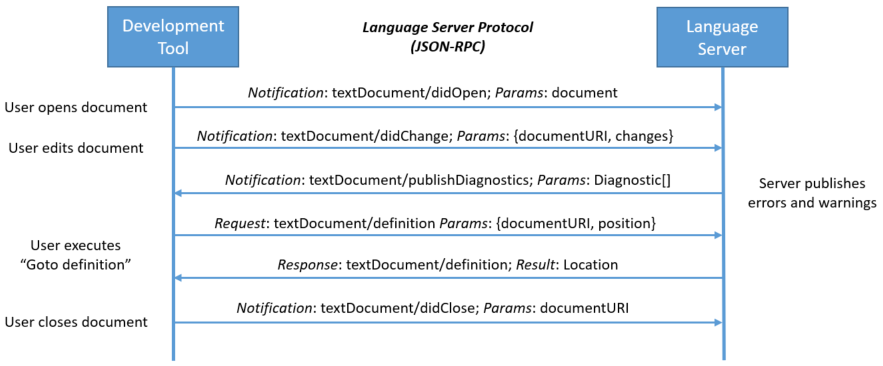
\includegraphics[width=\linewidth]{images/language-server-sequence.png}
        \caption{example for how a tool and a language server communicate during a routine editing session}
    \end{figure}
    
    Today, language servers for more than 50 languages exist\footnote{\url{https://microsoft.github.io/language-server-protocol/implementors/servers/} Sep. 2018}, including almost all popular programming and scripting languages\footnote{Regarding the popularity on GitHub in 2017 \url{https://octoverse.github.com/}}. Not all implementations support the full feature set defined in the \ac{lsp}. Typically, these language server implementations support exactly one language, but the \ac{lsp} allows multiple languages per server.
\chapter{Approach}
\label{cha:solution}

\section{How to get the relevant information out of Graal/Truffle}
\subsection{Parsing code}
\subsection{Mapping editor cursor position to Truffle source-section and node}
\subsection{Instrumentation}
\subsection{Challanges due to Truffles focus on performance}
    AST nodes lack relevant information, e.g. for refactoring. The language parsers are designed as fail-on-first-error. Only first syntax error is reported.
\section{Type harvesting evaluation strategies}
\todo{Is this already implementation?}
\subsection{Literals}
\subsection{Coverage data}
\subsection{Run-to-section}
\subsection{Globals}

\section{LSP features overview table}


\chapter{Implementation}
\label{cha:implementation}
\section{The lsp4j library}

\section{Architecture}
\subsection{Truffle-API + Graal-SDK}
\subsection{Launcher, Instrument, Server}
\subsection{Thread with entered Context}

\section{What a TruffleLanguage needs to implement}
    % https://www.graalvm.org/docs/graalvm-as-a-platform/implement-instrument/
    The onInputValue method can be used in combination with source section filters to intercept very fine-grained execution events such as intermediate values used by language expressions. The intermediate values that are accessible to the instrumentation framework greatly depend on the instrumentation support provided by each language.
    % https://www.graalvm.org/docs/graalvm-as-a-platform/implement-instrument/
\subsection{Expression- and Statement-Tag}
\subsection{findSourceLocation()}
\subsection{findTopScopes()}
\subsection{findLocalScopes()}
\subsection{findMetaObject()}
\subsection{getCompletionTriggerCharacters()}
\subsection{boxPrimitive()}
\subsection{parseInline()}
\subsection{GetSignature custom message}

\section{LSP features implementation - TextDocumentService}
% \subsection{completion}
% \subsection{hover}
% \subsection{signatureHelp}
% \subsection{definition}
% \subsection{typeDefinition}
% \subsection{implementation}
% \subsection{references}
% \subsection{documentHighlight}
% \subsection{documentSymbol}
% \subsection{codeAction}
% \subsection{codeLense}
% \subsection{formatting}
% \subsection{rangeFormatting}
% \subsection{onTypeFormatting}
% \subsection{rename}
% \subsection{didOpen}
% \subsection{didChange}
% \subsection{didClose}
% \subsection{didSave}
% \subsection{willSave}
% \subsection{willSaveWaitUntil}
% \subsection{documentLink}
% \subsection{documentLinkResolve}
% \subsection{documentColor}
% \subsection{colorPresentation}

\section{LSP features implementation - WorkspaceService}
% \subsection{executeCommand}
% \subsection{symbol}
% \subsection{didChangeConfiguration}
% \subsection{didChangeWatchedFiles}
% \subsection{didChangeWorkspaceFolders}

\section{LSP client config}
\subsection{VSCode extension exmaple + Limitations}

\chapter{Experience report}
\label{cha:evaluation}
\section{Between IDE and Language Workbench}
    Language Workbench focus/aim: Efficient language (DSL) development, performance is not main focus
    vs. Graal/Truffle aim: Efficient execution

    Assumption: Language Workbenches use static information only, our Truffle-based solution uses dynamic type information
\section{Completion response time}

\section{Limitations} 
\todo{own chapter? or in cha:implementation?}
\subsection{VSCode: Need to define supported languages in extension}
\subsection{VSCode: Syntax highlighting defined at client-side}
\subsection{Server: Only TCP (connecting to already running server), no std-in/-out impl}
\subsection{Truffle: Only first syntax error is reported. Lang parsers fail on first error}


\chapter{Related Work}
\label{cha:relatedwork}

\section{Graal}
\cite{seaton2014debugging}
\section{Squimera}
\cite{niephaus2018live}
\cite{niephaus2017squeak}
\section{Language Workbenches}
\cite{erdweg2013state}
\section{Run-time type collection}
\cite{haupt2011type}


\chapter{Conclusion and Future Work}
\label{cha:conclusion}



\printbibliography
\clearpage
\appendix
% !TEX root = Stolpe_2018_Thesis.tex
% !TEX encoding = UTF-8
%% ggf:
% \part{Appendix}
% \label{part:appendix}

\chapter{First Unimportant stuff.}
\label{cha:first-unimp-stuff}

\blindtext
%%% Local Variables:
%%% mode: latex
%%% TeX-master: "Stolpe_2018_Thesis"
%%% coding: utf-8
%%% End:

\backmatter
\markboth{}\relax

% BAMA-O (2009) §24.8
%  Am Schluss der Arbeit hat die/der Kandidat/in  zu versichern, dass 
%  sie/er sie selbstständig verfasst sowie keine anderen Quellen und 
%  Hilfsmittel als die angegebenen benutzt hat.
% BAMA-O (2013) §30.6
%  Am Schluss der Arbeit hat die Kandidatin bzw. der Kandidat zu versichern,
%  dass sie bzw. er die Arbeit selbstständig verfasst und keine anderen
%  Quellen und Hilfsmittel als die angegebenen benutzt hat.
\defaultstatement
\end{document}
%%% Local Variables:
%%% mode: latex
%%% TeX-master: t
%%% coding: utf-8
%%% End:
